% !TEX program = xelatex
% !TEX options = -interaction=nonstopmode -synctex=1 -output-directory=build "%DOC%"

\documentclass[a4paper, final]{article}
\usepackage{amsmath}
\usepackage{amssymb}
\usepackage{fontspec}
\setmainfont{Times New Roman}
\newfontfamily\cyrillicfonttt{Courier New}
\usepackage[14pt]{extsizes}

\usepackage{polyglossia}
\setdefaultlanguage{russian}

\usepackage[left=20mm, top=20mm, right=20mm, bottom=20mm, footskip=10mm]{geometry}
\usepackage{ragged2e}
\usepackage{indentfirst}
\usepackage{hyperref}
\usepackage{graphicx}
\usepackage{tikz}
\usepackage{caption}
\usepackage{subcaption}
\usepackage{xcolor}
\usepackage{listings}
\usepackage{algorithm}
\usepackage{algorithmic}
\usepackage{soul}
\usepackage{pdflscape}
\usepackage{longtable}
\usepackage{array}
\usepackage{ragged2e}
\usepackage{caption}
\usepackage{makecell}   % перенос строк в заголовках
\usepackage{graphicx}  
\usepackage{tabularx}
\usepackage{booktabs}
\usepackage{pdfpages}


\definecolor{codegray}{gray}{0.95}
\definecolor{codered}{rgb}{0.6,0,0}
\definecolor{codeblue}{rgb}{0,0,0.6}
\definecolor{codegreen}{rgb}{0,0.5,0}

\lstdefinestyle{common}{
  basicstyle=\ttfamily\small,
  backgroundcolor=\color{codegray},
  frame=single,
  numbers=left,
  numberstyle=\tiny\color{gray},
  stepnumber=1,
  numbersep=6pt,
  showspaces=false,
  showstringspaces=false,
  showtabs=false,
  tabsize=2,
  breaklines=true,
  breakatwhitespace=true,
  captionpos=b,
  keywordstyle=\color{codeblue}\bfseries,
  commentstyle=\color{codegreen}\itshape,
  stringstyle=\color{codered}
}

% \lstdefinestyle{cstyle}{
%     style=common,
%     language=C++,
%     extendedchars=true
% }

\lstdefinestyle{bashstyle}{
  style=common,
  language=bash
}

\linespread{0.98}

\definecolor{link_color}{HTML}{0000EE}

\hypersetup{
    colorlinks=true, 
    linkcolor=link_color, 
    urlcolor=link_color, 
    citecolor=link_color
}

% \lstdefinestyle{cstyle}{
%     style=common,
%     language=C++,
%     inputencoding=utf8,
%     extendedchars=true,
%     keywordstyle=\color{blue}\bfseries,
%     commentstyle=\color{gray}\itshape,
%     stringstyle=\color{orange},
%     showstringspaces=false,
%     breaklines=true
% }

\lstdefinestyle{cstyle}{
    style=common,
    language=C++,
    inputencoding=utf8,
    extendedchars=true,
    keepspaces=true,
    columns=fullflexible,
	    literate={а}{{\selectfont\char224}}1
             {б}{{\selectfont\char225}}1
             {в}{{\selectfont\char226}}1
             {г}{{\selectfont\char227}}1
             {д}{{\selectfont\char228}}1
             {е}{{\selectfont\char229}}1
             {ё}{{\"e}}1
             {ж}{{\selectfont\char230}}1
             {з}{{\selectfont\char231}}1
             {и}{{\selectfont\char232}}1
             {й}{{\selectfont\char233}}1
             {к}{{\selectfont\char234}}1
             {л}{{\selectfont\char235}}1
             {м}{{\selectfont\char236}}1
             {н}{{\selectfont\char237}}1
             {о}{{\selectfont\char238}}1
             {п}{{\selectfont\char239}}1
             {р}{{\selectfont\char240}}1
             {с}{{\selectfont\char241}}1
             {т}{{\selectfont\char242}}1
             {у}{{\selectfont\char243}}1
             {ф}{{\selectfont\char244}}1
             {х}{{\selectfont\char245}}1
             {ц}{{\selectfont\char246}}1
             {ч}{{\selectfont\char247}}1
             {ш}{{\selectfont\char248}}1
             {щ}{{\selectfont\char249}}1
             {ъ}{{\selectfont\char250}}1
             {ы}{{\selectfont\char251}}1
             {ь}{{\selectfont\char252}}1
             {э}{{\selectfont\char253}}1
             {ю}{{\selectfont\char254}}1
             {я}{{\selectfont\char255}}1
             {А}{{\selectfont\char192}}1
             {Б}{{\selectfont\char193}}1
             {В}{{\selectfont\char194}}1
             {Г}{{\selectfont\char195}}1
             {Д}{{\selectfont\char196}}1
             {Е}{{\selectfont\char197}}1
             {Ё}{{\"E}}1
             {Ж}{{\selectfont\char198}}1
             {З}{{\selectfont\char199}}1
             {И}{{\selectfont\char200}}1
             {Й}{{\selectfont\char201}}1
             {К}{{\selectfont\char202}}1
             {Л}{{\selectfont\char203}}1
             {М}{{\selectfont\char204}}1
             {Н}{{\selectfont\char205}}1
             {О}{{\selectfont\char206}}1
             {П}{{\selectfont\char207}}1
             {Р}{{\selectfont\char208}}1
             {С}{{\selectfont\char209}}1
             {Т}{{\selectfont\char210}}1
             {У}{{\selectfont\char211}}1
             {Ф}{{\selectfont\char212}}1
             {Х}{{\selectfont\char213}}1
             {Ц}{{\selectfont\char214}}1
             {Ч}{{\selectfont\char215}}1
             {Ш}{{\selectfont\char216}}1
             {Щ}{{\selectfont\char217}}1
             {Ъ}{{\selectfont\char218}}1
             {Ы}{{\selectfont\char219}}1
             {Ь}{{\selectfont\char220}}1
             {Э}{{\selectfont\char221}}1
             {Ю}{{\selectfont\char222}}1
             {Я}{{\selectfont\char223}}1,
}

\lstdefinelanguage{Go}{
  morekeywords={break,case,chan,const,continue,default,defer,else,fallthrough,for,func,go,goto,if,import,interface,map,package,range,return,select,struct,switch,type,var,nil,true,false,error,string,int,int8,int16,int32,int64,uint,uint8,uint16,uint32,uint64,float32,float64,bool,byte,rune,make,len,cap,append,copy,close,delete,new,panic,recover},
  sensitive=true,
  morecomment=[l]{//},
  morecomment=[s]{/*}{*/},
  morestring=[b]",
columns=fullflexible,
	    literate={а}{{\selectfont\char224}}1
             {б}{{\selectfont\char225}}1
             {в}{{\selectfont\char226}}1
             {г}{{\selectfont\char227}}1
             {д}{{\selectfont\char228}}1
             {е}{{\selectfont\char229}}1
             {ё}{{\"e}}1
             {ж}{{\selectfont\char230}}1
             {з}{{\selectfont\char231}}1
             {и}{{\selectfont\char232}}1
             {й}{{\selectfont\char233}}1
             {к}{{\selectfont\char234}}1
             {л}{{\selectfont\char235}}1
             {м}{{\selectfont\char236}}1
             {н}{{\selectfont\char237}}1
             {о}{{\selectfont\char238}}1
             {п}{{\selectfont\char239}}1
             {р}{{\selectfont\char240}}1
             {с}{{\selectfont\char241}}1
             {т}{{\selectfont\char242}}1
             {у}{{\selectfont\char243}}1
             {ф}{{\selectfont\char244}}1
             {х}{{\selectfont\char245}}1
             {ц}{{\selectfont\char246}}1
             {ч}{{\selectfont\char247}}1
             {ш}{{\selectfont\char248}}1
             {щ}{{\selectfont\char249}}1
             {ъ}{{\selectfont\char250}}1
             {ы}{{\selectfont\char251}}1
             {ь}{{\selectfont\char252}}1
             {э}{{\selectfont\char253}}1
             {ю}{{\selectfont\char254}}1
             {я}{{\selectfont\char255}}1
             {А}{{\selectfont\char192}}1
             {Б}{{\selectfont\char193}}1
             {В}{{\selectfont\char194}}1
             {Г}{{\selectfont\char195}}1
             {Д}{{\selectfont\char196}}1
             {Е}{{\selectfont\char197}}1
             {Ё}{{\"E}}1
             {Ж}{{\selectfont\char198}}1
             {З}{{\selectfont\char199}}1
             {И}{{\selectfont\char200}}1
             {Й}{{\selectfont\char201}}1
             {К}{{\selectfont\char202}}1
             {Л}{{\selectfont\char203}}1
             {М}{{\selectfont\char204}}1
             {Н}{{\selectfont\char205}}1
             {О}{{\selectfont\char206}}1
             {П}{{\selectfont\char207}}1
             {Р}{{\selectfont\char208}}1
             {С}{{\selectfont\char209}}1
             {Т}{{\selectfont\char210}}1
             {У}{{\selectfont\char211}}1
             {Ф}{{\selectfont\char212}}1
             {Х}{{\selectfont\char213}}1
             {Ц}{{\selectfont\char214}}1
             {Ч}{{\selectfont\char215}}1
             {Ш}{{\selectfont\char216}}1
             {Щ}{{\selectfont\char217}}1
             {Ъ}{{\selectfont\char218}}1
             {Ы}{{\selectfont\char219}}1
             {Ь}{{\selectfont\char220}}1
             {Э}{{\selectfont\char221}}1
             {Ю}{{\selectfont\char222}}1
             {Я}{{\selectfont\char223}}1,
}

\definecolor{sqlblue}{RGB}{0,0,180}
\definecolor{sqlfunc}{RGB}{128,0,128}
\definecolor{sqlstr}{RGB}{163,21,21}
\definecolor{sqlcomment}{RGB}{0,128,0}

\lstdefinelanguage{SQL}{
  morekeywords=[1]{
    SELECT, FROM, WHERE, JOIN, LEFT, RIGHT, INNER, OUTER, FULL, CROSS,
    ON, AS, AND, OR, NOT, IN, EXISTS, BETWEEN, LIKE, IS, NULL,
    GROUP, BY, ORDER, HAVING, DISTINCT, UNION, ALL, EXCEPT, INTERSECT,
    INSERT, INTO, VALUES, UPDATE, SET, DELETE, TRUNCATE,
    CREATE, TABLE, INDEX, VIEW, DROP, ALTER, ADD, COLUMN,
    PRIMARY, KEY, FOREIGN, REFERENCES, UNIQUE, DEFAULT, CHECK,
    WITH, RECURSIVE, CASE, WHEN, THEN, ELSE, END,
    LIMIT, OFFSET, ASC, DESC, RETURNING
  },
  morekeywords=[2]{
    COUNT, MAX, MIN, SUM, AVG, COALESCE, NULLIF, GREATEST, LEAST,
    NOW, CURRENT_DATE, CURRENT_TIMESTAMP, EXTRACT, DATE_TRUNC,
    LOWER, UPPER, TRIM, LENGTH, SUBSTRING, CONCAT, REPLACE,
    CAST, ROUND, FLOOR, CEIL, ABS, MOD
  },
  sensitive=false,
  morecomment=[l]{--},
  morecomment=[s]{/*}{*/},
  morestring=[b]',
  morestring=[b]",
}

\lstdefinestyle{sqlstyle}{
    style=common,
    language=SQL,
    keepspaces=true,
    columns=fullflexible,
    keywordstyle=[1]\color{sqlblue}\bfseries,
    keywordstyle=[2]\color{sqlfunc}\bfseries,
    commentstyle=\color{sqlcomment}\itshape,
    stringstyle=\color{sqlstr},
    literate={а}{{\selectfont\char224}}1
             {б}{{\selectfont\char225}}1
             {в}{{\selectfont\char226}}1
             {г}{{\selectfont\char227}}1
             {д}{{\selectfont\char228}}1
             {е}{{\selectfont\char229}}1
             {ё}{{\"e}}1
             {ж}{{\selectfont\char230}}1
             {з}{{\selectfont\char231}}1
             {и}{{\selectfont\char232}}1
             {й}{{\selectfont\char233}}1
             {к}{{\selectfont\char234}}1
             {л}{{\selectfont\char235}}1
             {м}{{\selectfont\char236}}1
             {н}{{\selectfont\char237}}1
             {о}{{\selectfont\char238}}1
             {п}{{\selectfont\char239}}1
             {р}{{\selectfont\char240}}1
             {с}{{\selectfont\char241}}1
             {т}{{\selectfont\char242}}1
             {у}{{\selectfont\char243}}1
             {ф}{{\selectfont\char244}}1
             {х}{{\selectfont\char245}}1
             {ц}{{\selectfont\char246}}1
             {ч}{{\selectfont\char247}}1
             {ш}{{\selectfont\char248}}1
             {щ}{{\selectfont\char249}}1
             {ъ}{{\selectfont\char250}}1
             {ы}{{\selectfont\char251}}1
             {ь}{{\selectfont\char252}}1
             {э}{{\selectfont\char253}}1
             {ю}{{\selectfont\char254}}1
             {я}{{\selectfont\char255}}1
             {А}{{\selectfont\char192}}1
             {Б}{{\selectfont\char193}}1
             {В}{{\selectfont\char194}}1
             {Г}{{\selectfont\char195}}1
             {Д}{{\selectfont\char196}}1
             {Е}{{\selectfont\char197}}1
             {Ё}{{\"E}}1
             {Ж}{{\selectfont\char198}}1
             {З}{{\selectfont\char199}}1
             {И}{{\selectfont\char200}}1
             {Й}{{\selectfont\char201}}1
             {К}{{\selectfont\char202}}1
             {Л}{{\selectfont\char203}}1
             {М}{{\selectfont\char204}}1
             {Н}{{\selectfont\char205}}1
             {О}{{\selectfont\char206}}1
             {П}{{\selectfont\char207}}1
             {Р}{{\selectfont\char208}}1
             {С}{{\selectfont\char209}}1
             {Т}{{\selectfont\char210}}1
             {У}{{\selectfont\char211}}1
             {Ф}{{\selectfont\char212}}1
             {Х}{{\selectfont\char213}}1
             {Ц}{{\selectfont\char214}}1
             {Ч}{{\selectfont\char215}}1
             {Ш}{{\selectfont\char216}}1
             {Щ}{{\selectfont\char217}}1
             {Ъ}{{\selectfont\char218}}1
             {Ы}{{\selectfont\char219}}1
             {Ь}{{\selectfont\char220}}1
             {Э}{{\selectfont\char221}}1
             {Ю}{{\selectfont\char222}}1
             {Я}{{\selectfont\char223}}1
             {—}{{---}}1,
}

\lstdefinestyle{gostyle}{
    style=common,
    language=Go,
    keepspaces=true,
    columns=fullflexible,
	    columns=fullflexible,
	    literate={а}{{\selectfont\char224}}1
             {б}{{\selectfont\char225}}1
             {в}{{\selectfont\char226}}1
             {г}{{\selectfont\char227}}1
             {д}{{\selectfont\char228}}1
             {е}{{\selectfont\char229}}1
             {ё}{{\"e}}1
             {ж}{{\selectfont\char230}}1
             {з}{{\selectfont\char231}}1
             {и}{{\selectfont\char232}}1
             {й}{{\selectfont\char233}}1
             {к}{{\selectfont\char234}}1
             {л}{{\selectfont\char235}}1
             {м}{{\selectfont\char236}}1
             {н}{{\selectfont\char237}}1
             {о}{{\selectfont\char238}}1
             {п}{{\selectfont\char239}}1
             {р}{{\selectfont\char240}}1
             {с}{{\selectfont\char241}}1
             {т}{{\selectfont\char242}}1
             {у}{{\selectfont\char243}}1
             {ф}{{\selectfont\char244}}1
             {х}{{\selectfont\char245}}1
             {ц}{{\selectfont\char246}}1
             {ч}{{\selectfont\char247}}1
             {ш}{{\selectfont\char248}}1
             {щ}{{\selectfont\char249}}1
             {ъ}{{\selectfont\char250}}1
             {ы}{{\selectfont\char251}}1
             {ь}{{\selectfont\char252}}1
             {э}{{\selectfont\char253}}1
             {ю}{{\selectfont\char254}}1
             {я}{{\selectfont\char255}}1
             {А}{{\selectfont\char192}}1
             {Б}{{\selectfont\char193}}1
             {В}{{\selectfont\char194}}1
             {Г}{{\selectfont\char195}}1
             {Д}{{\selectfont\char196}}1
             {Е}{{\selectfont\char197}}1
             {Ё}{{\"E}}1
             {Ж}{{\selectfont\char198}}1
             {З}{{\selectfont\char199}}1
             {И}{{\selectfont\char200}}1
             {Й}{{\selectfont\char201}}1
             {К}{{\selectfont\char202}}1
             {Л}{{\selectfont\char203}}1
             {М}{{\selectfont\char204}}1
             {Н}{{\selectfont\char205}}1
             {О}{{\selectfont\char206}}1
             {П}{{\selectfont\char207}}1
             {Р}{{\selectfont\char208}}1
             {С}{{\selectfont\char209}}1
             {Т}{{\selectfont\char210}}1
             {У}{{\selectfont\char211}}1
             {Ф}{{\selectfont\char212}}1
             {Х}{{\selectfont\char213}}1
             {Ц}{{\selectfont\char214}}1
             {Ч}{{\selectfont\char215}}1
             {Ш}{{\selectfont\char216}}1
             {Щ}{{\selectfont\char217}}1
             {Ъ}{{\selectfont\char218}}1
             {Ы}{{\selectfont\char219}}1
             {Ь}{{\selectfont\char220}}1
             {Э}{{\selectfont\char221}}1
             {Ю}{{\selectfont\char222}}1
             {Я}{{\selectfont\char223}}1,
}

\begin{document}
\emergencystretch=2em

% ТИТУЛЬНЫЙ ЛИСТ
{\thispagestyle{empty}
\begin{center}
    \hfill\\[10pt]
    МИНИСТЕРСТВО НАУКИ И ВЫСШЕГО ОБРАЗОВАНИЯ РОССИЙСКОЙ ФЕДЕРАЦИИ\\[5pt]
    Федеральное государственное автономное образовательное учреждение высшего образования\\
    «Санкт-Петербургский политехнический университет Петра Великого»\\[10pt]
    Институт компьютерных наук и кибербезопасности\\[5pt]
    Высшая школа технологий искусственного интеллекта\\[5pt]
    Направление: 02.03.01 Математика и компьютерные науки\\[35pt]

    {\large Сети ЭВМ и телекоммуникации компьютерных сетей}\\[12pt]
    {\Large Отчет о выполнении лабораторной работы № 1}\\[10pt]
    {\large Вариант 24}
\end{center}

\vspace{120pt}

\begin{tabular*}{460pt}{@{\extracolsep{\fill}} l r}
    Выполнил студент группы\\5130201/40102 & Адиатуллин Т. Р. \quad \line(1,0){100}\\[18pt]
    Проверил преподаватель & Мулюха В. А. \quad \line(1,0){100}\\
    & \\
    & \\
    & \guillemotleft \line(1,0){30} \guillemotright \line(1,0){100} \, 2026 \,г.
\end{tabular*}

\vfill
\begin{center}
    Санкт-Петербург, 2026
\end{center}
\newpage
}

\tableofcontents
\newpage

\section{Задание 1. Разбиение сети на подсети}
Исходную IP-сеть разделите на 5 подсетей с заданным числом адресов в подсетях 

\textbf{Дано.} 

Адрес: 20.40.80.160;

Маска: 255.255.255.192;

Требования к подсетям: Ровно в одной подсети должно быть 16 адресов.

\textbf{Решение.} Маска задаёт сеть /26. Адрес 20.40.80.160 находится внутри сети 20.40.80.128/26. Всего в этой сети 64 адреса: от 20.40.80.128 до 20.40.80.191.

Разобью 64 адреса на пять блоков: 32, 16, 8, 4 и 4 адреса. В сумме получается $32+16+8+4+4=64$. Поэтому вся исходная сеть будет использована, и только один блок будет содержать 16 адресов. Результат показан в таблице.

\begin{table}[ht]
\centering
\small
\caption{Распределение исходной сети на подсети}
\begin{tabular}{|c|c|c|c|}
\hline
№ & Адрес подсети / маска & Диапазон адресов устройств & Всего адресов \\
\hline
1 & \makecell{20.40.80.128/27\\255.255.255.224} & 20.40.80.129--20.40.80.158 & 32 \\
\hline
2 & \makecell{20.40.80.160/28\\255.255.255.240} & 20.40.80.161--20.40.80.174 & 16 \\
\hline
3 & \makecell{20.40.80.176/29\\255.255.255.248} & 20.40.80.177--20.40.80.182 & 8 \\
\hline
4 & \makecell{20.40.80.184/30\\255.255.255.252} & 20.40.80.185--20.40.80.186 & 4 \\
\hline
5 & \makecell{20.40.80.188/30\\255.255.255.252} & 20.40.80.189--20.40.80.190 & 4 \\
\hline
\end{tabular}
\end{table}

В таблице указан диапазон адресов, которые можно выдать устройствам. Первый и последний адрес каждого блока зарезервированы для адреса сети и широковещательного адреса. Поэтому во второй подсети из 16 адресов устройствам доступны 14.

\newpage
\section{Задание 2. Вычисление скорости Wi-Fi соединений}

Используя таблицу вычислить MCS, модуляцию и соотношение скорости соединения WiFi для двух устройств.


\begin{figure}[H]
    \centering
    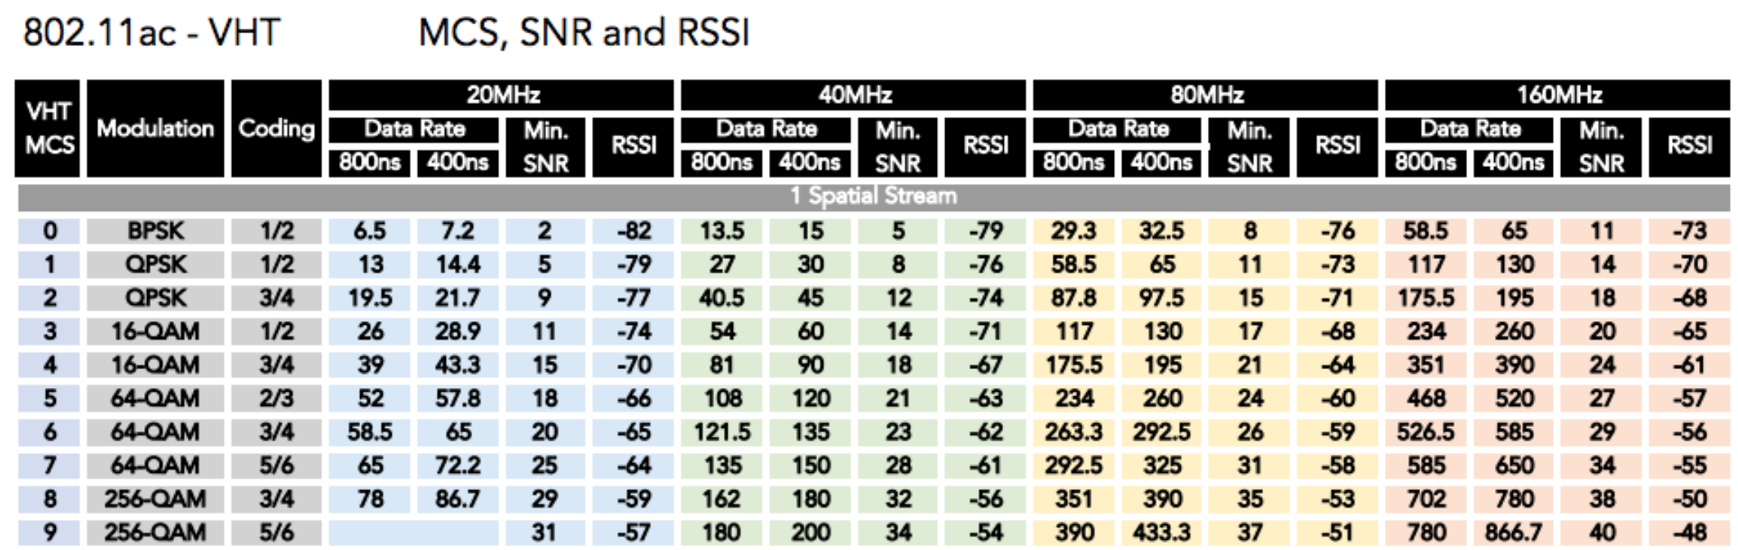
\includegraphics[width=0.9\linewidth]{myPhoto/mcs-table.png}
    \caption{Таблица режимов 802.11ac: MCS, RSSI и Data Rate}
    \label{tab:mcs-table}
\end{figure}

\textbf{Дано.} 

Два устройства(A и B) подключены к одному маршрутизатору 802.11ac. 

Параметры соединения (полоса и количество потоков настраиваются по наименьшим значениям, допустимым для данной силы сигнала) 


Устройство A: RSSI $=-58$ dBm, полоса 160 МГц, MIMO 4. 

Устройство B: RSSI $=-65{,}5$ dBm, полоса 20 МГц, MIMO 2.

\textbf{Решение.} По RSSI выбираю самый высокий MCS, для которого хватает уровня сигнала. В столбцах Data Rate указана скорость передачи. Подписи 800 нс и 400 нс показывают значение GI (защитного интервала).

\subsection{Устройство A}

Для MCS 4 (16-QAM, кодирование 3/4) нужен сигнал не слабее $-61$ dBm. Для MCS 5 нужен сигнал не слабее $-57$ dBm. У устройства A сигнал $-58$ dBm, поэтому ему подходит MCS 4, но не MCS 5.

\begin{samepage}
В столбцах Data Rate для одного потока указаны скорости: 351 Мбит/с при GI 800 нс и 390 Мбит/с при GI 400 нс. У устройства A четыре потока, поэтому умножаю скорость на 4.
\[
R_A(800\text{ нс})=351\cdot4=1404\text{ Мбит/с},\qquad
R_A(400\text{ нс})=390\cdot4=1560\text{ Мбит/с}.
\]
\end{samepage}

\subsection{Устройство Б}

Для MCS 5 (64-QAM, кодирование 2/3) нужен сигнал не слабее $-66$ dBm, а для MCS 6 -- не слабее $-65$ dBm. У устройства Б сигнал $-65{,}5$ dBm, значит, ему подходит MCS 5.

В столбцах Data Rate для одного потока указаны скорости: 52 Мбит/с при GI 800 нс и 57,8 Мбит/с при GI 400 нс. У устройства Б два потока, поэтому умножаю скорость на 2.
\[
R_{\text{Б}}(800\text{ нс})=52\cdot2=104\text{ Мбит/с},\qquad
R_{\text{Б}}(400\text{ нс})=57{,}8\cdot2=115{,}6\text{ Мбит/с}.
\]

Оба устройства подключены к одному маршрутизатору, поэтому скорость каждого уменьшаю в два раза:
\[
R_A: 702\text{ Мбит/с (800 нс)},\quad 780\text{ Мбит/с (400 нс)};
\]
\[
R_{\text{Б}}: 52\text{ Мбит/с (800 нс)},\quad 57{,}8\text{ Мбит/с (400 нс)}.
\]

Сравню скорости устройств A и Б:
\[
\frac{702}{52}\approx13{,}5,\qquad \frac{780}{57{,}8}\approx13{,}49.
\]
Получается, устройство A примерно в 13,5 раза быстрее устройства Б.

\newpage

\section{Задание 3. Расчёт времени передачи файла}

Сколько времени потребуется на передачу файла размером «А» МБайт, при размере кадра канального уровня «B» Байт и доле повторно передаваемых пакетов «С»/1000.

\begin{itemize}
	\item В качестве протокола канального уровня используется Ethernet DIX, на сетевом уровне – IPv4, размеры заголовков транспортного и прикладного уровней вместе – 26 байт. Физический уровень 100BaseT.
	\item Время на передачу одного пакета данных составляет 89 мс. Задержка при повторной передаче пакета составляет 300 мс без учета времени повторной передачи.
	\item Повторная передача осуществляется после передачи 1000/«С» пакетов с округлением в большую сторону до ближайшего целого
\end{itemize}

\textbf{Дано.} 
\begin{itemize}
	\item А = 71 Мбайт
	\item В = 1145 Байт
	\item С = 8.44
\end{itemize}


\textbf{Решение.} Сначала посчитаю, сколько байт занимает служебная информация в каждом кадре:
\begin{itemize}
    \item заголовок Ethernet DIX -- 14 байт;
    \item FCS Ethernet -- 4 байта;
    \item заголовок IPv4 -- 20 байт;
    \item заголовки транспортного и прикладного уровней -- 26 байт.
\end{itemize}
Всего это $14+4+20+26=64$ байта. Значит, для данных остаётся:
\[
B_{\text{пол}}=1145-64=1081\text{ байт}.
\]

В расчёте принимаю 1 Мбайт равным $1024^2$ байта. Тогда файл содержит:
\[
A=71\cdot1024^2=74\,448\,896\text{ байт}.
\]
Чтобы передать весь файл, понадобится столько кадров (округляю вверх):
\[
N=\left\lceil\frac{74\,448\,896}{1081}\right\rceil=68\,871.
\]

Повтор происходит через такое число пакетов (округляю вверх):
\[
I=\left\lceil\frac{1000}{8{,}44}\right\rceil=119\text{ пакетов}.
\]
Число повторов, после которых добавляется задержка:
\[
N_{\text{соб}}=\left\lceil\frac{68\,871}{119}\right\rceil=579.
\]
По доле $C/1000$ число повторно передаваемых пакетов равно (округляю вверх):
\[
N_{\text{повт}}=\left\lceil68\,871\cdot\frac{8{,}44}{1000}\right\rceil=582.
\]

Время передачи всех исходных пакетов:
\[
T_{\text{исх}}=68\,871\cdot89=6\,129\,519\text{ мс}.
\]
Общее время задержек перед повторами:
\[
T_{\text{зад}}=579\cdot300=173\,700\text{ мс}.
\]
Время передачи повторных пакетов:
\[
T_{\text{повт}}=582\cdot89=51\,798\text{ мс}.
\]

Время генерации и передачи одного кадра при скорости 100 Мбит/с:
\[
t_{\text{кадр}}=\frac{1145\cdot8}{100\cdot10^6}\text{ с}=0{,}0916\text{ мс}.
\]
Для 68 871 исходных кадров это $68\,871\cdot0{,}0916=6308{,}58$ мс. Время отправки повторных пакетов уже посчитано отдельно выше.

Складываю время исходной передачи, задержек, повторных пакетов и передачи кадров:
\[
T=T_{\text{исх}}+T_{\text{зад}}+T_{\text{повт}}+T_{\text{кадр}}
=6\,361\,325{,}58\text{ мс}.
\]
\[
T\approx6361{,}33\text{ с}\approx1\text{ ч }46\text{ мин }1\text{ с}.
\]

Для полной передачи потребуется примерно 1 час 46 минут и 1 секунда.
\end{document}
